\section{Question 2}
\subsection{Part A}
\begin{figure}[H]
	\centering
	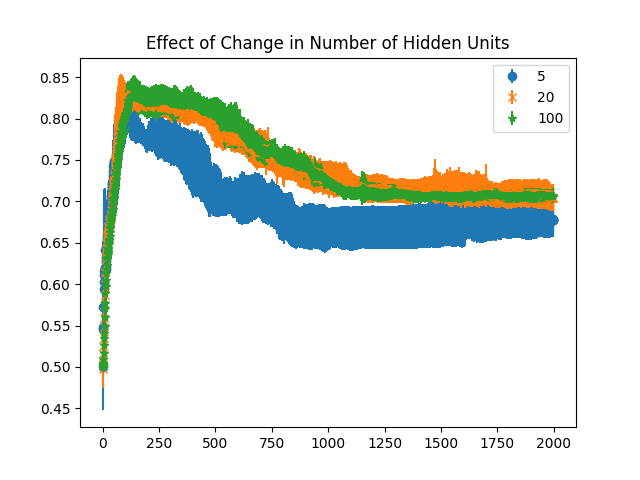
\includegraphics[width=0.6\textwidth]{../train2/hidden_units.png}
	\caption{Effect of changing number of hidden units}
\end{figure}

\subsection{Part B}
\begin{figure}[H]
	\centering
	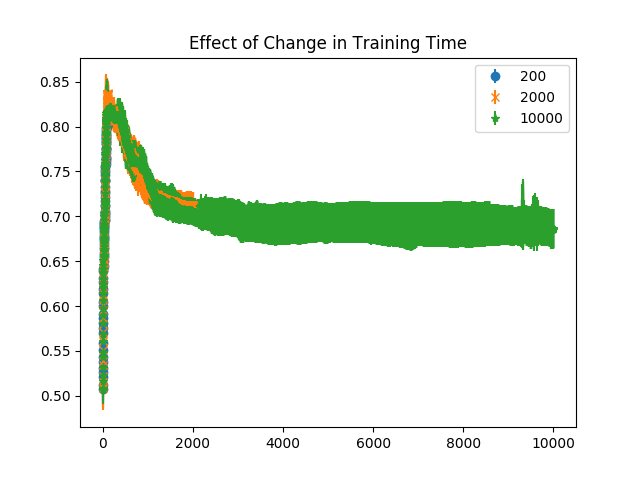
\includegraphics[width=0.6\textwidth]{../train2/epochs.png}
	\caption{Effect of changing traning time}
\end{figure}

\subsection{Part C}
\begin{figure}[H]
	\centering
	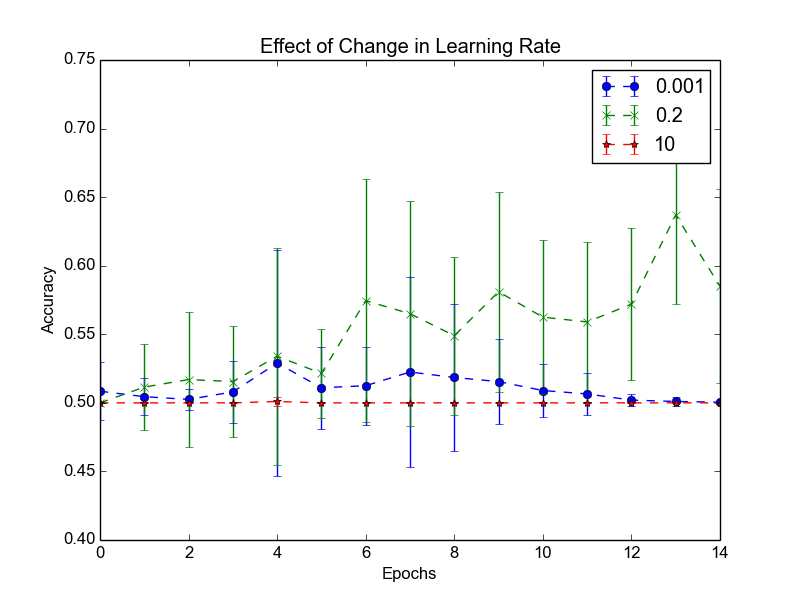
\includegraphics[width=0.6\textwidth]{../train2/learning_rate.png}
	\caption{Effect of changing learning rate}
\end{figure}

\subsection{Part E}
\begin{figure}[H]
	\centering
	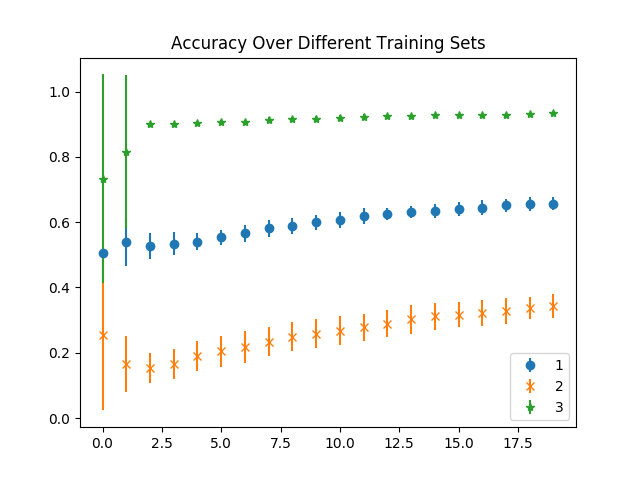
\includegraphics[width=0.6\textwidth]{../train2/data_sets.png}
	\caption{Effect of classifier on different test data sets}
\end{figure}